\chapter{\label{ch:5-result}Results}

\section{Digital literacy index - RQ1}
Figure \ref{fig:screeplot_rq1} is the screeplot derived from the PCA analysis, which shows the proportion of variance explained by each principal component. Following the three rules of thumb (Zelterman, 2015, p. 212) described in Section 4.3.1.2, this study selects the first principal component (PC1) as the digital literacy index. The specific steps are as follows: i) principal components are selected in sequence (i.e., from left to right); ii) according to the screeplot, PC1 is a clear upward outlier among all principal components; iii) PC1 explains around 25\% of the total variance, which surpasses the 20\% threshold. 

\begin{figure}
    \centering
    \caption{Screeplot of PCA - RQ1}
    \label{fig:screeplot_rq1}
    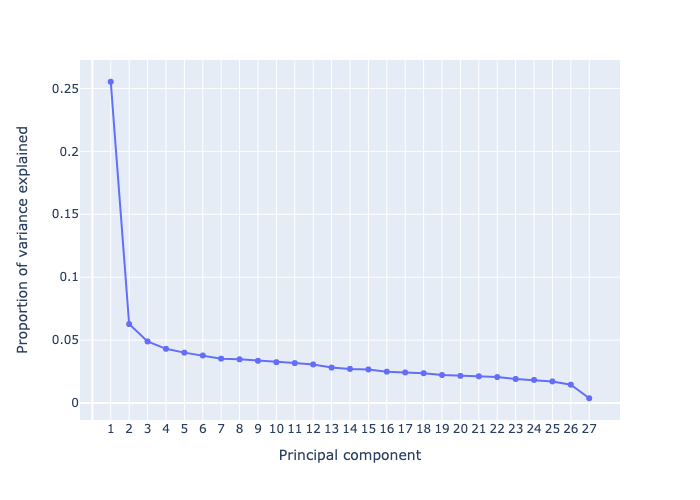
\includegraphics[width=\textwidth]{figures/pca_screeplot_q1.png}
\end{figure}

Further examination of PC1's loadings (see Table \ref{tab:pc1_loadings_rq1}) supports its appropriateness as a digital literacy index. The loading for frequency of Internet usage is positive, meaning that respondents with larger PC1 scores use the Internet less frequently. All loadings of hardware literacy are negative, suggesting that respondents with larger PC1 scores use fewer devices to access the Internet. All loadings of software literacy (except for ``no online activities”, which is positive) are negative, indicating that respondents with larger PC1 scores do fewer online activities and are more likely to do no online activities. These loadings consistently point to the direction that large PC1 scores correspond to lower digital literacy, thereby validating the use of PC1 as the digital literacy index.

\begin{table}[h!]
    \centering
    \caption{Loadings of PC1 - RQ1}
    \label{tab:pc1_loadings_rq1}
    \begin{tabular}{llc}
        \toprule
        Feature & Description & Loading \\
        \midrule
        \textbf{Frequency of Internet usage} & 1 = every day, 6 = never & 0.280 \\
        & & \\
        \textbf{Hardware literacy} (devices) & 1 = yes, 0 = no & \\
        desktop &  & -0.094 \\
        laptop &  & -0.137 \\
        tablet &  & -0.121 \\
        smartphone &  & -0.245 \\
        other devices &  & -0.039 \\
        & & \\
        \textbf{Software literacy} (activities) & 1 = yes, 0 = no & \\
        emails &  & -0.258 \\
        video calls &  & -0.226 \\
        finding information &  & -0.218 \\
        finances &  & -0.247 \\
        shopping &  & -0.257 \\
        selling &  & -0.106 \\
        social networking &  & -0.178 \\
        news &  & -0.223 \\
        TV/radio &  & -0.219 \\
        music &  & -0.178 \\
        games &  & -0.082 \\
        e-books &  & -0.124 \\
        job application &  & -0.071 \\
        government services &  & -0.216 \\
        checking travel times &  & -0.248 \\
        satellite navigation &  & -0.229 \\
        buying public transport tickets &  & -0.167 \\
        booking a taxi &  & -0.088 \\
        finding local amenities &  & -0.231 \\
        controlling household appliances &  & -0.124 \\
        no online activities &  & 0.249 \\
        \bottomrule
    \end{tabular}
\end{table}

To enhance interpretability, this study adjusts the PC1 scores by reversing their signs, where now larger values indicate greater digital literacy. Subsequently, PC1 scores are dichotomised to get the explanatory variable: respondents in the lower quartile (bottom 25\%) are categorised as having low digital literacy, coded as 0, while those in the upper quartile (top 25\%) are categorised as having high digital literacy, coded as 1. Table \ref{tab: explanatory_variable_rq1} shows the distribution of the dichotomised explanatory variable.

\begin{table}[h!]
    \centering
    \caption{Distribution of explanatory variable - RQ1}
    \label{tab:explanatory_variable_rq1}
    \begin{tabular}{lc}
        \toprule
        Digital literacy & Count \\
        \midrule
        Low & 994 \\
        High & 994 \\
        \bottomrule
    \end{tabular}
\end{table}

\section{Descriptive statistics - RQ1}
Table \ref{tab: desc_stats_rq1} presents the descriptive statistics by digital literacy. 

\begin{sidewaystable}[h!]
    \centering
    \footnotesize
    \caption{Descriptive statistics by digital literacy - RQ1}
    \label{tab:desc_stats_rq1}
    \begin{tabular}{llcc}
        \toprule
        Variables & Description & \multicolumn{2}{c}{Digital literacy} \\
        & & Low (N = 994) & High (N = 994) \\
        \midrule
        \textbf{Outcome variables} & & & \\
        Self-rated health & 1 = excellent, 5 = poor & 3.002 & 2.337 \\
        Physical health & 1 = yes, 0 = no & \\
        \hspace{0.5cm} High blood pressure &  & 0.468 & 0.308 \\
        \hspace{0.5cm} High cholesterol &  & 0.471 & 0.304 \\
        \hspace{0.5cm} Diabetes &  & 0.141 & 0.070 \\
        \hspace{0.5cm} Asthma &  & 0.114 & 0.100 \\
        \hspace{0.5cm} Arthritis &  & 0.477 & 0.318 \\
        \hspace{0.5cm} Cancer &  & 0.054 & 0.011 \\
        Mental health & & \\
        \hspace{0.5cm} Depression score & 0 = no symptom, 8 = all symptoms & 1.474 & 1.013 \\
        \hspace{0.5cm} Anxiety disorder & 1 = yes, 0 = no & 0.084 & 0.102 \\
        \hspace{0.5cm} Mood swings & 1 = yes, 0 = no & 0.020 & 0.014 \\
        & & & \\
        \textbf{Control variables} & & & \\
        Age &  & 74.408 & 64.655 \\
        Gender & 0 = male, 1 = female & 0.595 & 0.495 \\
        Marital status & proportion & & \\
        \hspace{0.5cm} Single &  & 0.064 & 0.079 \\
        \hspace{0.5cm} Married &  & 0.512 & 0.596 \\
        \hspace{0.5cm} Remarried &  & 0.100 & 0.151 \\
        \hspace{0.5cm} Separated &  & 0.008 & 0.009 \\
        \hspace{0.5cm} Divorced &  & 0.118 & 0.109 \\
        \hspace{0.5cm} Widowed &  & 0.198 & 0.056 \\
        Ethnicity & 0 = white, 1 = non-white & 0.023 & 0.048 \\
        Age left full-time education & 2 = never went to school, 8 = 19 or over & 5.101 & 6.704 \\
        Highest educational level & proportion & & \\
        \hspace{0.5cm} Degree or equivalent &  & 0.121 & 0.480 \\
        \hspace{0.5cm} HE below degree &  & 0.143 & 0.146 \\
        \hspace{0.5cm} A-level or equivalent &  & 0.098 & 0.142 \\
        \hspace{0.5cm} O-level or equivalent &  & 0.255 & 0.161 \\
        \hspace{0.5cm} CSE or equivalent &  & 0.050 & 0.005 \\
        \hspace{0.5cm} Foreign/other qualification &  & 0.097 & 0.044 \\
        \hspace{0.5cm} No qualification &  & 0.236 & 0.023 \\
        Employment status & 1 = in paid employment, 0 = not & 0.131 & 0.441 \\
        Household income (decile) & 0 = 1st decile, 9 = 10th decile & 3.263 & 5.753 \\
        Deprivation index & 0 = least deprived, 9 = most & 0.424 & 0.286 \\
        Memory & 1 = excellent, 5 = poor & 3.339 & 2.874 \\
        Numeracy index & 0 = lowest numeracy ability, 5 = highest & 3.423 & 4.217 \\
        Comprehension index & 0 = lowest comprehension ability, 4 = highest & 3.446 & 3.883 \\
        \bottomrule
    \end{tabular}
\end{sidewaystable}

In terms of outcome variables, respondents with high digital literacy consistently exhibit superior health outcomes across three different dimensions. Specifically, as for self-rated health, the average level for respondents with high digital literacy is 2.337 (i.e., ``very good"), while those with lower digital literacy have an average score of 3.002 (i.e., ``good"). As for physical health, individuals with high digital literacy are less likely to be diagnosed with all six surveyed diseases than their less digitally literate counterparts. As for mental health, those with higher digital literacy levels report fewer depressive symptoms and are less prone to mood swings. However, it is noted that respondents with high digital literacy are more likely to be diagnosed with anxiety disorders, with a minimal difference of 0.018. Given the consistency of other health outcomes, this slight discrepancy is likely attributable to statistical randomness.

In terms of control variables, respondents with high digital literacy also possess socio-economic advantages that can lead to both higher digital literacy and better health outcomes. Specifically, Individuals with high digital literacy tend to be younger, predominantly male, and more likely to be married or remarried rather than divorced or widowed. They are typically non-White, have left full-time education at an older age, and possess higher educational qualifications. Furthermore, they are more likely to be employed, earn a higher household income, experience lower levels of deprivation, and demonstrate enhanced memory, numeracy, and comprehension skills compared to their less digitally literate counterparts.

It is important to recognise that these correlations between digital literacy and health outcomes, as observed in the descriptive statistics, do not imply causation. As detailed earlier, while respondents with high digital literacy generally display better health outcomes, they also possess socio-economic advantages that could independently contribute to both higher digital literacy and better health. This observation suggests the potential for omitted variable bias, as highlighted in Section 2.3.2. Another possible bias highlighted in Section 2.3.2 is simultaneity bias, as the correlation between digital literacy and health can be driven by health instead of digital literacy. Thus, conducting a thorough causal analysis that adequately addresses these potential biases is crucial for understanding the true impact of digital literacy on health outcomes.

\section{Main results - RQ1}
This study adopts an identification strategy that accounts for both simultaneity bias and omitted variable bias. Table \ref{tab:iptw} presents the IPTW estimate of the average treatment effect (ATE) of digital literacy on older adults' health outcomes. In short, higher digital literacy leads to better health outcomes in 6 out of the 10 variables examined, spanning across all three health dimensions. 

\begin{table}[h!]
    \centering
    \caption{IPTW estimate - Effect of digital literacy on health}
    \label{tab:iptw}
    \begin{threeparttable}
        \begin{tabular}{llc}
            \toprule
            Outcome & Description & IPTW \\
            \midrule
            Self-rated health & 1 = excellent, 5 = poor & \textbf{-0.326}*** \\
            & & [-7.353] \\
            & & \\
            Physical health & 1 = yes, 0 = no & \\
            High blood pressure &  & 0.002 \\
            &  & [0.065] \\
            High cholesterol &  & \textbf{-0.067}** \\
            &  & [-2.809] \\
            Diabetes &  & \textbf{-0.034}* \\
            &  & [-2.307] \\
            Asthma &  & \textbf{-0.042}** \\
            &  & [-2.787] \\
            Arthritis &  & -0.018 \\
            &  & [-0.758] \\
            Cancer &  & \textbf{-0.031}*** \\
            &  & [-4.068] \\
            & & \\
            Mental health & & \\
            Depression score & 0 = no symptom, 8 = all symptoms & \textbf{-0.292}*** \\
            & & [-3.887] \\
            Anxiety disorder & 1 = yes, 0 = no  & -0.018 \\
            &  & [-1.245] \\
            Mood swings & 1 = yes, 0 = no  & 0.009 \\
            &  & [1.757] \\
            \bottomrule
        \end{tabular}
        \begin{tablenotes}
            \footnotesize
            \item Notes: *** $p < 0.001$, ** $p < 0.01$, * $p < 0.05$. t-statistics are reported in square brackets.
        \end{tablenotes}
    \end{threeparttable}
\end{table}

As for self-rated health, the IPTW estimate is -0.326, meaning that with other factors held constant, high digital literacy improves self-rated health by 0.326 points, moving it closer to ``excellent". This effect is statistically significant at the 0.001 level.

As for physical health, with other factors held constant, high digital literacy leads to a 6.7 percentage points decrease in the likelihood of being diagnosed with high cholesterol, a 3.4 percentage points decrease for diabetes, a 4.2 percentage points decrease for asthma, and a 3.1 percentage points for cancer. The effects on these four diseases are statistically significant. High digital literacy also leads to a 1.8 percentage points decrease for arthritis, but this effect is not statistically significant. Interestingly, the IPTW estimate for high blood pressure is positive 0.002, but the effect size is minimal and is not statistically different from zero. This suggests that the estimate is likely due to statistical randomness rather than a genuine effect of high digital literacy on increasing the incidence of high blood pressure.

As for mental health, with other factors held constant, high digital literacy reduces the number of depressive symptoms by 0.292, and this effect is statistically significant at 0.001 level. High digital literacy also leads to a 1.8 percentage points decrease in the likelihood of being diagnosed with anxiety disorder, but this effect is not statistically significant. Interestingly, the IPTW estimate for mood swings is positive 0.009, but again this effect size is minimal and is not statistically different from zero. This suggests that the estimate is likely due to statistical randomness rather than a genuine effect of high digital literacy on increasing the incidence of mood swings.

In summary, the IPTW results confirm the hypothesis for the first research question, demonstrating that high digital literacy contributes to improved health outcomes among older adults. This beneficial effect is evident 6 out of the 10 health outcomes examined, which span across all three health dimensions. Specifically, the six health outcomes showing statistical significance are self-rated health, physical health (high cholesterol, diabetes, asthma, and cancer), and mental health (depression).

\section{Robustness checks - RQ1}

\subsection{Strong ignorability}
As discussed in Section 4.4.2, one critical assumption of the IPTW method is strong ignorability. To evaluate the robustness of the IPTW estimates against potential violations of this assumption, this study conducts sensitivity analyses on health outcomes that demonstrated statistical significance. The outcomes of these analyses are depicted in Figure \ref{fig:sense}. Points on or above with the red dashed line indicate scenarios where an uncontrolled confounder would negate the observed effect.

\begin{figure}
    \centering
    \caption{Sensitivity analysis}
    \label{fig:sense}
    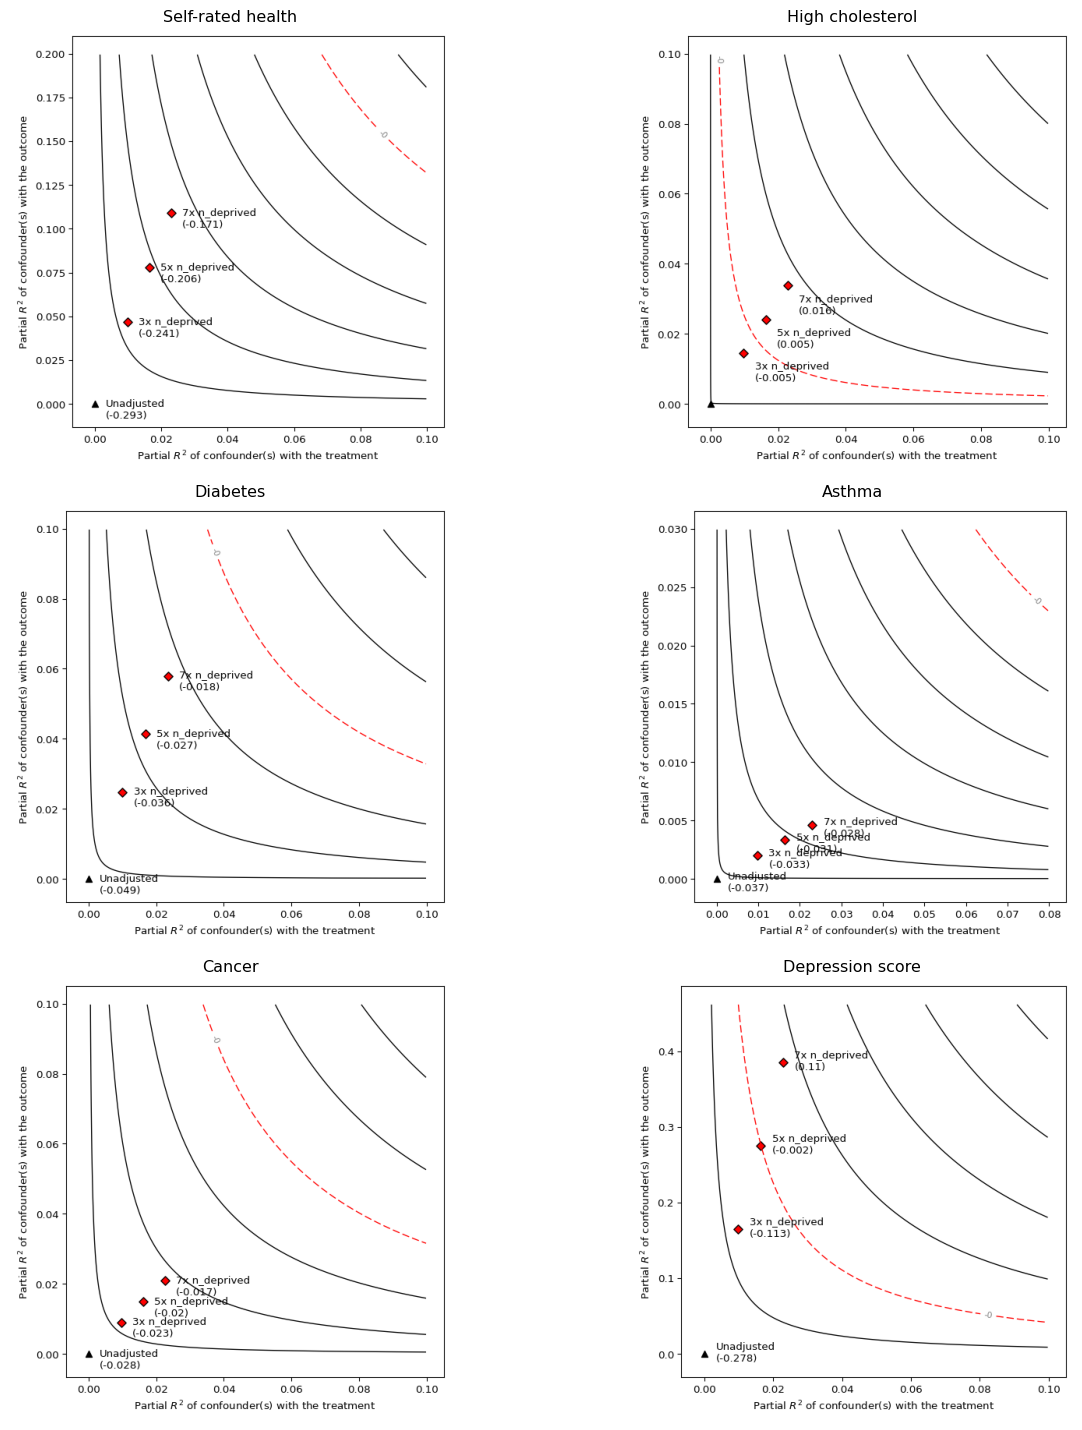
\includegraphics[width=\textwidth]{figures/sensitivity.png}
    \caption*{\footnotesize Notes: Points that reach the red dashed line indicate that the observed effect is nullified by the uncontrolled confounder.}
\end{figure}

For self-rated health, diabetes, asthma, and cancer, the results from the sensitivity analysis underscore the robustness of their IPTW estimates. As illustrated, their corresponding 7x points all fall below the red dash line, meaning that even an uncontrolled confounder exerting seven times the effect of deprivation — a factor extensively documented as a critical confounder in the literature on digital literacy and health outcomes (Zelterman, 2015, p. 212) — fails to invalidate the observed relationships. The improbability of encountering an uncontrolled confounder with such a disproportionately high impact strengthens the robustness of the identified causal effects of digital literacy on self-rated health, diabetes, asthma, and cancer.

Regarding depression, the figure shows that the 5x point is on the red dash line, meaning that an uncontrolled confounder with an impact five times greater than that of deprivation could nullify the observed effect. Similarly regarding high cholesterol, the figure shows that the red dash line lies between the 3x and 5x point, meaning that that an uncontrolled confounder with an impact approximately four times greater than that of deprivation could nullify observed relationship. Although a fourfold or fivefold effect appears less extreme than a sevenfold effect, identifying such a potent uncontrolled confounder remains highly improbable given that deprivation is already a very impactful confounder. 

In summary, while the strong ignorability assumption remains inherently untestable, this sensitivity analysis provides compelling evidence of the robustness of IPTW estimates, particularly for self-rated health, diabetes, asthma, and cancer. These findings affirm that higher digital literacy contributes to improved health outcomes across all three dimensions for older adults.

\subsection{Positivity}
As discussed in Section 4.4.2, another critical assumption of the IPTW method is positivity. To evaluate the robustness of the IPTW estimates against potential violations of this assumption, this study implements the two rules of thumb recommended by Cole and Hernan (2008). For the first rule, the calculated mean of the stabilised weights is 0.942, indicating minimal deviation from the ideal value of one. For the second rule, the minimum and maximum values of the stabilised weights are 0.463 and 21.29 respectively, neither too extreme. These results suggest that the treatment assignment is well-balanced across the levels of confounders within the sample, supporting the integrity of the positivity assumption in this study.

\section{Digital literacy index - RQ2}
As mentioned in Section 4.6.1, this study conducts separate PCA analyses for Wave 9 and 10 to address the potential contamination of group assignment. Figure \ref{fig:screeplot_rq2} is the screeplot derived from the two PCA analyses, which shows the proportion of variance explained by each principal component. 

\begin{figure}
    \centering
    \caption{Screeplot of PCA - RQ2}
    \label{fig:screeplot_rq2}
    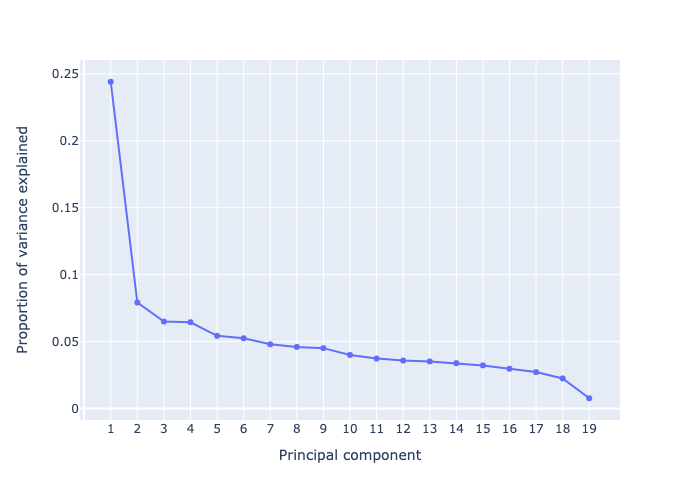
\includegraphics[width=\textwidth]{figures/pca_screeplot_q2.png}
\end{figure}

For Wave 9, following the three rules of thumb (Zelterman, 2015) described in Section 4.3.1.2, this study selects PC1 as the digital literacy index for Wave 9. The specific steps are as follows: i) principal components are selected in sequence (i.e., from left to right); ii) according to the screeplot, PC1 is a clear upward outlier among all principal components; iii) PC1 explains around 25\% of the total variance, which surpasses the 20\% threshold. 

Further examination of PC1's loadings (see Table \ref{tab:pc1_loadings_w9_rq2}) supports its appropriateness as a digital literacy index. The loading for frequency of Internet usage is positive, meaning that respondents with larger PC1 scores use the Internet less frequently. All loadings of hardware literacy are negative, suggesting that respondents with larger PC1 scores use fewer devices to access the Internet. All loadings of software literacy (except for “no online activities”, which is positive) are negative, indicating that respondents with larger PC1 scores do fewer online activities and are more likely to do no online activities. These loadings consistently point to the direction that large PC1 scores correspond to lower digital literacy, thereby validating the use of PC1 as the digital literacy index.


\begin{sidewaystable}[h!]
        \centering
        \caption{Loadings of PC1 - RQ2}
        \label{tab:pc1_loadings_rq2}
    
        \begin{subtable}[t]{0.4\textwidth}
            \centering
            \scriptsize
            \caption{Wave 9}
            \label{tab:pc1_loadings_w9_rq2}
            \begin{tabular}{llc}
                \toprule
                Feature & Description & Loading \\
                \midrule
                \textbf{Frequency of Internet usage} & 1 = every day, 6 = never & 0.357 \\
                & & \\
                \textbf{Hardware literacy} (devices) & 1 = yes, 0 = no & \\
                desktop &  & -0.124 \\
                laptop &  & -0.129 \\
                tablet &  & -0.143 \\
                smartphone &  & -0.243 \\
                other devices &  & -0.019 \\
                do not use any device &  & 0.320 \\
                & & \\
                \textbf{Software literacy} (activities) & 1 = yes, 0 = no & \\
                emails &  & -0.308 \\
                video calls &  & -0.176 \\
                finding information (learning) &  & -0.213 \\
                finding information (health) &  & -0.261 \\
                finances &  & -0.250 \\
                shopping &  & -0.269 \\
                selling &  & -0.107 \\
                social networking &  & -0.176 \\
                creating content &  & -0.084 \\
                news &  & -0.215 \\
                music &  & -0.214 \\
                games &  & -0.082 \\
                job application &  & -0.067 \\
                government services &  & -0.162 \\
                other online activities &  & -0.021 \\
                no online activities &  & 0.324 \\
                \bottomrule
            \end{tabular}
        \end{subtable}
        \hfil
        \begin{subtable}[t]{0.4\textwidth}
            \centering
            \scriptsize
            \caption{Wave 10}
            \label{tab:pc1_loadings_w10_rq2}
            \begin{tabular}{llc}
                \toprule
                Feature & Description & Loading \\
                \midrule
                \textbf{Frequency of Internet usage} & 1 = every day, 6 = never & 0.278 \\
                & & \\
                \textbf{Hardware literacy} (devices) & 1 = yes, 0 = no & \\
                desktop &  & -0.091 \\
                laptop &  & -0.134 \\
                tablet &  & -0.114 \\
                smartphone &  & -0.245 \\
                other devices &  & -0.042 \\
                & & \\
                \textbf{Software literacy} (activities) & 1 = yes, 0 = no & \\
                emails &  & -0.255 \\
                video calls &  & -0.224 \\
                finding information &  & -0.217 \\
                finances &  & -0.247 \\
                shopping &  & -0.255 \\
                selling &  & -0.107 \\
                social networking &  & -0.177 \\
                news &  & -0.225 \\
                TV/radio &  & -0.221 \\
                music &  & -0.183 \\
                games &  & -0.079 \\
                e-books &  & -0.124 \\
                job application &  & -0.072 \\
                government services &  & -0.218 \\
                checking travel times &  & -0.251 \\
                satellite navigation &  & -0.234 \\
                buying public transport tickets &  & -0.173 \\
                booking a taxi &  & -0.087 \\
                finding local amenities &  & -0.231 \\
                controlling household appliances &  & -0.126 \\
                no online activities &  & 0.243 \\
                \bottomrule
            \end{tabular}
        \end{subtable}
\end{sidewaystable}

The PCA results for Wave 10 closely mirror those of Wave 9, with similar patterns observed in both the screeplot and the loadings. Therefore, PC1 is also chosen as the digital literacy index for Wave 10.

To enhance interpretability, this study adjusts both PC1 scores by reversing their signs, where now larger values indicate greater digital literacy. Subsequently, PC1 scores are dichotomised to get the explanatory variable for Wave 9 and 10 respectively: respondents in the lower quartile (bottom 25\%) are categorised as having low digital literacy, coded as 0, while those in the upper quartile (top 25\%) are categorised as having high digital literacy, coded as 1. Table \ref{tab: explanatory_variable_rq2} shows the distribution of the dichotomised explanatory variable for Wave 9 and 10.

\begin{table}[h!]
    \centering
    \caption{Distribution of explanatory variable - RQ2}
    \label{tab:explanatory_variable_rq2}
    \begin{tabular}{lcc}
        \toprule
         & Wave 10 - Low & Wave 10 - High \\
        \midrule
        Wave 9 - Low & 658 & 3 \\
        Wave 9 - High & 10 & 565 \\
        \bottomrule
    \end{tabular}
\end{table}

As illustrated, there are 13 respondents who experienced changes in their level of digital literacy between Wave 9 and 10, leading to contamination of group assignment. This finding justifies the identification strategy detailed in Section 4.6.1, which only selects respondents who did not have any changes in their level of digital literacy across waves.

\section{Descriptive statistics - RQ2}
Figure \ref{fig:desc_stats_rq2} presents respondents’ health trends by the dichotomised digital literacy explanatory variable (i.e., low and high). As a reminder, Wave 9 was conducted before the COVID-19 pandemic and Wave 10 was conducted during the pandemic. For most of the variables examined, respondents with high digital literacy have better health outcomes than those with low digital literacy, as evidenced by the non-overlapping 95\% confidence intervals.

\begin{figure}
    \centering
    \caption{Health trends by digital literacy}
    \label{fig:desc_stats_rq2}
    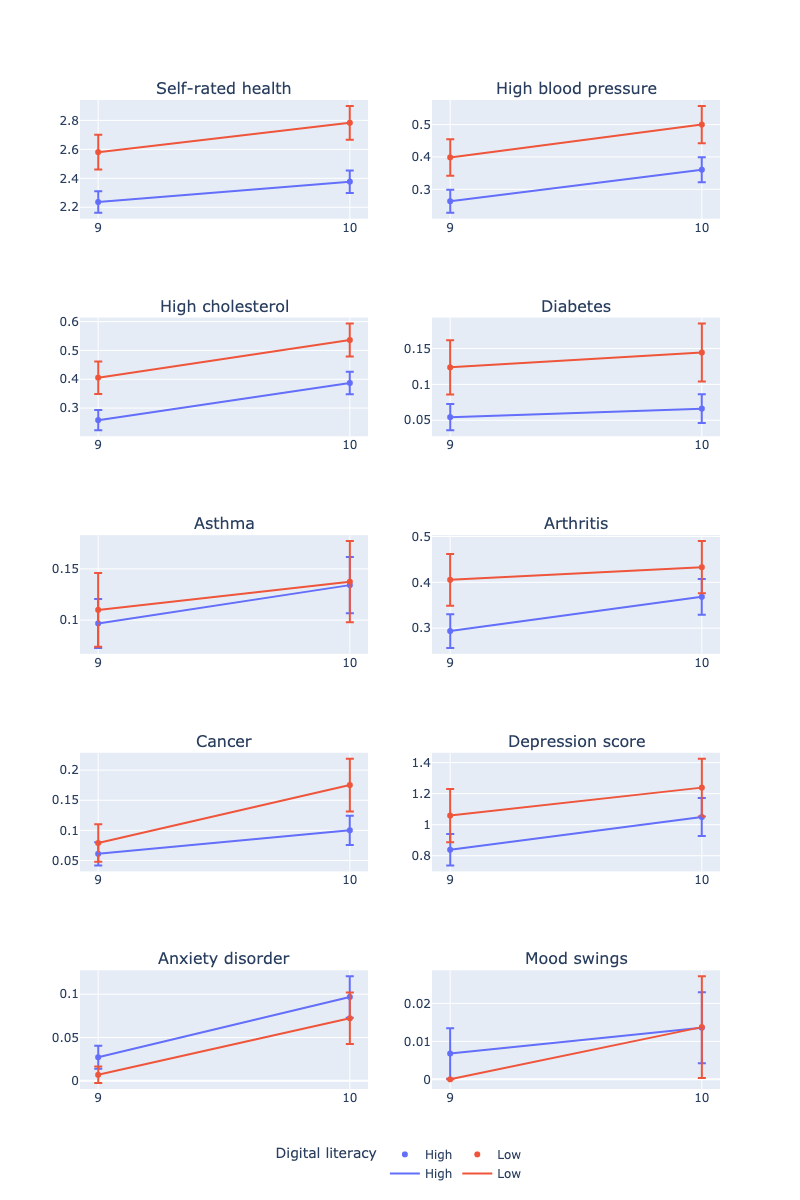
\includegraphics[width=\textwidth]{figures/desc_stats_q2.png}
    \caption*{Notes: The error bars represent 95\% confidence intervals.}
\end{figure}

As for self-rated health, a significant pre-existing difference was noted at Wave 9, where respondents with high digital literacy reported better health than those with low digital literacy. This disparity persisted into Wave 10, as indicated by parallel trends in the figure.

As for physical health, respondents with high digital literacy at Wave 9 showed a significantly lower likelihood of being diagnosed with high blood pressure, high cholesterol, diabetes, and arthritis compared to those with low digital literacy. These disparities persisted into Wave 10, as indicated by parallel trends in the figure. However, for asthma and cancer, the figure shows overlapping confidence intervals between the two groups at both waves, suggesting no significant differences in the incidence of asthma and cancer between respondents with low and high digital literacy.

As for mental health, for depression, a significant difference was observed in depression at Wave 9, with respondents having high digital literacy experiencing fewer depressive symptoms. This disparity persisted into Wave 10, as indicated by parallel trends in the figure. However, for anxiety disorder and mood swings, the figure shows overlapping confidence intervals between the two groups at both waves, suggesting no significant differences in the incidence of anxiety disorder and mood swings between respondents with low and high digital literacy.

It is important to recognise that these statistics are descriptive and does not imply that increased digitalisation does not exert any impact on the health inequalities between older adults with low and high digital literacy. As discussed in Section 4.6, relying on a simple DiD comparison assumes the validity of parallel trends, an assumption that is very unlikely to hold in this context due to significant socio-economic differences among respondents, as detailed in Table \ref{tab: desc_stats_rq1}. Thus, a more thorough causal analysis, which carefully addresses potential biases, is essential to accurately determine the impacts of increased digitalisation on health disparities among older adults with low and high digital literacy.

\section{Main results - RQ2}
This study adopts an identification strategy that accounts for both the potential contamination of group assignment and the potential violation of the parallel trends assumption. Table \ref{tab:did} presents the Matching DiD estimate of the impact of increased digitalisation on the health disparities between older adults with low and high digital literacy. In short, increased digitalisation has enlarged the health disparities in 3 out of the 10 variables examined, spanning across all three health dimensions. 

\begin{table}[h!]
    \centering
    \caption{DiD estimate - Impact of increased digitalisation on health disparities}
    \label{tab:did}
    \begin{threeparttable}
        \begin{tabular}{llc}
            \toprule
            Outcome & Description & Matching DiD \\
            \midrule
            Self-rated health & 1 = excellent, 5 = poor & \textbf{-0.207}*** \\
            &  & [-3.762] \\
            & & \\
            Physical health & 1 = yes, 0 = no & \\
            High blood pressure &  & -0.029 \\
            &  & [-1.523] \\
            High cholesterol &  & 0.002 \\
            &  & [0.061] \\
            Diabetes &  & \textbf{-0.044}*** \\
            &  & [-3.488] \\
            Asthma &  & 0.003 \\
            &  & [0.277] \\
            Arthritis &  & 0.01 \\
            &  & [0.562] \\
            Cancer &  & -0.026 \\
            &  & [-1.671] \\
            & & \\
            Mental health & & \\
            Depression score & 0 = no symptom, 8 = all symptoms & -0.115 \\
            &  & [-1.29] \\
            Anxiety disorder & 1 = yes, 0 = no & -0.011 \\
            &  & [-0.843] \\
            Mood swings & 1 = yes, 0 = no & \textbf{-0.013}** \\
            &  & [-2.845] \\
            \bottomrule
        \end{tabular}
        \begin{tablenotes}
            \footnotesize
            \item Notes: *** $p < 0.001$, ** $p < 0.01$, * $p < 0.05$. t-statistics are reported in square brackets.
        \end{tablenotes}
    \end{threeparttable}
\end{table}

As for self-rated health, the Matching DiD estimate is -0.207, meaning that increased digitalisation has enlarged the disparities in self-rated health. In more substantive words, if originally respondents with high digital literacy reported a self-rated health $x$ points better than those with low digital literacy, increased digitalisation has now increased this difference to $x + 0.207$ points. This effect is statistically significant at the 0.001 level. It is important to note that the respondents in this comparison are matched such that their only difference is the level of digital literacy; all other characteristics are the same.

As for physical health, the only disease showing statistical significance is diabetes, with a Matching DiD estimate of -0.044, meaning that increased digitalisation has enlarged the disparities in diabetes. In more substantive words, if originally respondents with high digital literacy were $x$ percentage points less likely to be diagnosed with diabetes, increased digitalisation has now increased this difference to $x + 4.4$ percentage points. Increased digitalisation also enlarged the disparities for high blood pressure and cancer (as shown by their negative coefficients), but these effects are not statistically significant. Interestingly, the estimates for high cholesterol, asthma, and arthritis are positive, but the effect sizes are minimal and not statistically different from zero, indicating that the observed shrinkage in disparities for these conditions are likely due to statistical randomness rather than a genuine effect of increased digitalisation on reducing health disparities.

As for mental health, the only disease showing statistical significance is mood swings, with a Matching DiD estimate of -0.013, meaning that increased digitalisation has enlarged the disparities in mood swings. In more substantive words, if originally respondents with high digital literacy were $x$ percentage points less likely to be diagnosed with mood swings, increased digitalisation has now increased this difference to $x + 1.3$ percentage points. For depression and anxiety disorder, increased digitalisation also enlarged the disparities as shown by their negative coefficients, but these effects are not statistically significant.

In summary, the Matching DiD estimates confirm the hypothesis for the second research question, demonstrating that increased digitalisation has exacerbated the health disparities between respondents with low and high digital literacy. This exacerbation is evident in 3 out of the 10 health outcomes examined, which spans across all three health dimensions. Specifically, the three health outcomes showing statistical significance are self-rated health, physical health (diabetes), and mental health (mood swings).
